\documentclass[11pt]{article}
\usepackage{graphicx}
\usepackage{hyperref}
\usepackage{appendix}
\usepackage{amsmath}
\usepackage{amsthm}
\usepackage{amssymb}
\usepackage{natbib}
\usepackage{float}
\usepackage{multirow}
\usepackage{commath}
\usepackage{booktabs}
\usepackage{subcaption}
\renewcommand{\arraystretch}{1.2}
\usepackage{siunitx}
\sisetup{detect-all}
\usepackage{listings}
\usepackage{color} %red, green, blue, yellow, cyan, magenta, black, white
\definecolor{mygreen}{RGB}{28,172,0} % color values Red, Green, Blue
\definecolor{mylilas}{RGB}{170,55,241}
\usepackage[a4paper,margin=20mm]{geometry}
\numberwithin{equation}{section}
\setlength{\parskip}{\baselineskip}
\setlength{\parindent}{0pt}
\hypersetup{
    colorlinks=true,
    linkcolor=black,
    filecolor=black,      
    urlcolor=black,
    citecolor=black
}
\urlstyle{same}
\lstset{language=Matlab,%
    %basicstyle=\color{red},
    breaklines=true,%
    morekeywords={matlab2tikz},
    keywordstyle=\color{blue},%
    morekeywords=[2]{1}, keywordstyle=[2]{\color{black}},
    identifierstyle=\color{black},%
    stringstyle=\color{mylilas},
    commentstyle=\color{mygreen},%
    showstringspaces=false,%without this there will be a symbol in the places where there is a space
    numbers=left,%
    numberstyle={\tiny \color{black}},% size of the numbers
    numbersep=9pt, % this defines how far the numbers are from the text
    emph=[1]{for,end,break},emphstyle=[1]\color{red}, %some words to emphasise
    %emph=[2]{word1,word2}, emphstyle=[2]{style},    
}
\begin{document}
\title{\textbf{UCL Mechanical Engineering 2021/2022}\\MECH0023 Coursework}
\author{RFLH9}
\date{\today}
\maketitle
\tableofcontents
\listoffigures
\section{Satellite model}
\subsection{Description of model and assumptions}
\subsection{Minimum thickness of beam}
\subsection{Amplitude of displacement for steady-state oscillation of the sensor during rocket function}
\subsection{Limitations of analysis}
\subsection{Manoeuvre}
\subsubsection{Description of obtaining sensor response to the thrust force}
\subsubsection{Dispalcement response}
\section{Linear modelling}
\subsection{Description of non-linearity between $y(t)$ \& $\theta(t)$}
The following function:
\begin{equation}
    \frac{\dif y\left( t\right)}{\dif t} = 150 \cos \left(\theta\left(t\right)\right) - 47
\end{equation}
has a non-linear relationship due to $\theta(t)$ being within a cosine function. There is also an offset value of $47$ which makes our relationship non-linear as well.
\subsection{Description of non-linear relationship in a real system}
An example of a non-linear relationship is car velocity and air resistance. Our input is the velocity of the car and our output is the drag force We can describe this relationship with the following equation.
\begin{align}
    F_D &= \frac{1}{2} \rho v^2 C_D A\\
    F_D &\propto v^2
\end{align}
The relationship between the drag force and velocity is proportionally squared. This means that as velocity increases, our drag force will increase by four times. Non-linearity can also come in the form as headwind or tailwind. Mathematically, this would be represented as a constant term ($B$) added to our equation. For example:
\begin{equation}
    F_D = \frac{1}{2} \rho v^2 C_D A + B\\
\end{equation}
\section{Linear model performance and stability}
\subsection{Unstable process + description of actuator switching on}
The transfer function, $G_p(s)$ is:
\begin{equation}
    G_p (s) = \frac{Y(s)}{V(s)} = \frac{1}{\left(s^2 - 81\right)}\frac{k}{\left(0.05s + 1\right)}
\end{equation}
By looking at the position of the roots ($s = 9$, $s = -9$, $s = -20$), we can check whether our system is unstable. We have a root at $s = 9$, which is on the positive side of the s-plane. This means that our whole system is unstable. 

Our poles lie on the real axis on the positive side of the s-plane. Hence, when we switch our voltage to \SI{5}{\volt}, we will find that our rudder angle will exponentially rise. We will not see any oscillation as our response will have no sine term. The rudder angle will continually to increase until it reaches its mechanical limit and potentially damage itself. The rudder angle may go in either direction (positive or negative/left or right) until it reaches this limit. 
\subsection{Root locus and effect of proportional control}
Using the following MATLAB code, the root locus of the system was plotted in Figure \ref{q3b}.
\lstinputlisting{./mCode/q3b.m}
\begin{figure}[H]
    \centering
    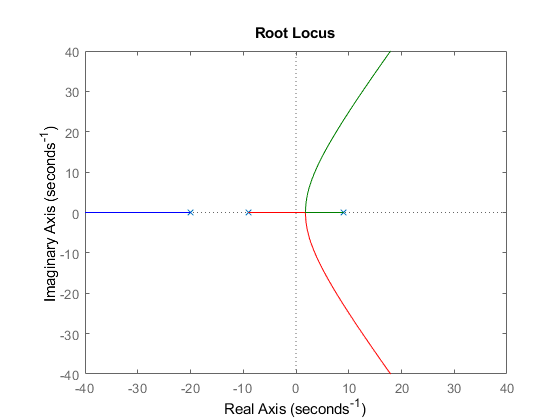
\includegraphics[width = 0.75\textwidth]{./img/q3b.png}
    \caption{Root locus of system.}
    \label{q3b}
\end{figure}
This root locus diagram shows us that the system would be unstable in closed-loop operation for all possible values of gain $K$, hence rendering proportional control ineffective for stabilising the system. 
\subsection{Negative velocity feedback controller}
\subsubsection{Plot of root locus}
Our new transfer function is:
\begin{equation}
    H_p(s) = \frac{k\left(s+8\right)}{0.05s^3 + s^2 -4.05s - 81}
\end{equation}
Using the following MATLAB code, the root locus of the system was plotted in Figure \ref{q3ci}.
\lstinputlisting{./mCode/q3ci.m}
\begin{figure}[H]
    \centering
    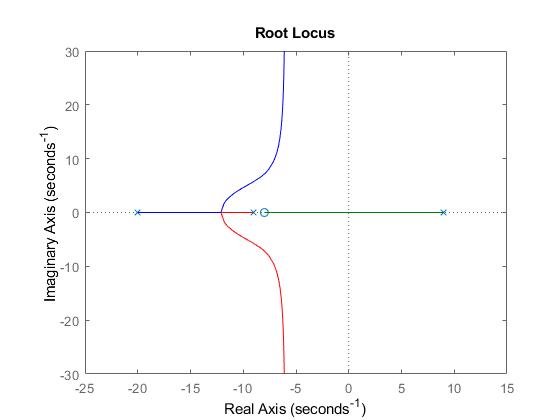
\includegraphics[width = 0.75\textwidth]{./img/q3ci.png}
    \caption{Root locus of system with negative velocity feedback controller.}
    \label{q3ci}
\end{figure}
\subsubsection{Areas where damping ratio is higher than 0.6 + damped natural frequency is higher than \SI{7}{\radian\per\second}}
We are given that our damping ratio must be at least 0.6 and that our damped natural frequency must be at least \SI{7}{\radian\per\second}:
\begin{gather}
    \zeta \geq 0.6\\
    \omega_d \geq 7
\end{gather}
Solving to find the minimum undamped natural frequency:
\begin{gather}
    \omega_n = \frac{\omega_d}{\sqrt{1 - \zeta^2}}\\
    \omega_n = \frac{7}{\sqrt{1-0.6^2}}\\
    \omega_n = 8.75
\end{gather}
Since the undamped and damped natural frequency are proportional, we know that:
\begin{equation}
    \omega_n \geq 8.75
\end{equation}
Using the following MATLAB code, the regions which fulfil the above constrains were plotted in Figure \ref{q3cii}.
\lstinputlisting{./mCode/q3cii.m}
\begin{figure}[H]
    \centering
    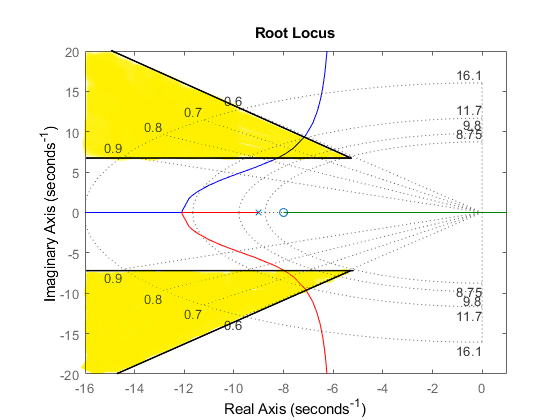
\includegraphics[width = 0.75\textwidth]{./img/q3cii2.png}
    \caption{Regions on root locus diagram where $\zeta \geq 0.6$ and $\omega_d \geq 7$.}
    \label{q3cii}
\end{figure}
\subsubsection{Range of $k$ where performance specifications are achieved}
By inspecting our MATLAB plots, we can find the gain values at any specified point.
\begin{figure}[H]
    \centering
    \begin{minipage}{.5\textwidth}
        \centering
        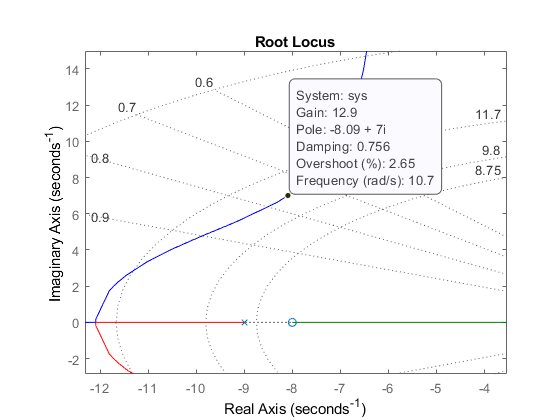
\includegraphics[width = \linewidth]{./img/q3ciii1.png}
        \caption{Minimum $k$ value.}
        \label{q3ciii1}
    \end{minipage}%
    \begin{minipage}{.5\textwidth}
        \centering
        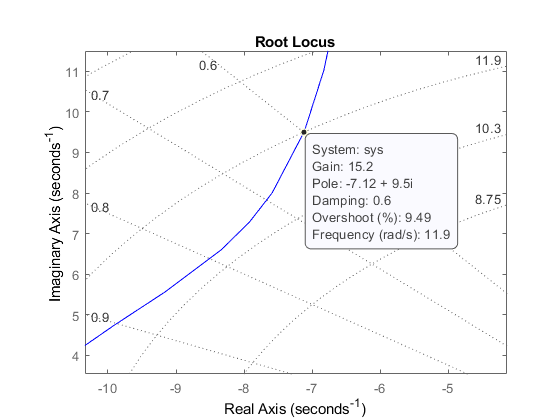
\includegraphics[width = \linewidth]{./img/q3ciii2.png}
        \caption{Maximum $k$ value.}
        \label{q3ciii2}
    \end{minipage}
\end{figure}
Here, we find that the maximum gain value that we can have is 15.2 at pole value $-7.12 + 9.5i$, limited by our damping ratio. For gains below 15.2, our pole position moves towards the real axis and away from the imaginary axis. The minimum gain value we can have is limited by the damped natural frequency and at a pole value of $-8.09 + 7i$, our gain is 12.9. Therefore:
\begin{equation}
    12.9 \leq k \leq 15.2
\end{equation}
\section{Controller techniques}
\subsection{Description of closed loop position control system}
The system I have chosen to describe is a drone autopilot system. The drone I have picked as part of this analysis is a DJI Mavic 3. This drone is used to take high quality aerial video footage, hence stability and control are important for this particular drone. In a simple case, let us try and make our drone hover in a fixed position above the ground (in a fixed reference frame). Our desired output response is to keep the drone's coordinates fixed. To further simplify our example, let us only consider the motion in the $z$-axis (altitude). 

The actuator is the motors attached to the drone propellers. The physical position to be controlled is the altitude of the drone. According to the drone specifications, the drone has a hovering accuracy range of $\pm\SI{0.1}{\metre}$ in the vertical (with Vision Positioning). Using GPS data, we have a lower hovering accuracy at $\pm \SI{0.5}{\metre}$ \citep{dji}. As this is a video recording drone, the ability to stay at a fixed altitude and to not `drift' is important to prevent the footage from looking shaky/blurry/distracting. 
\subsection{Specify disturbances}
\section{Inverted pendulum}
\subsection{Identification and description of assumptions and limitations for the model of a rotary inverted pendulum}
\subsection{Moving rocket to final position}
\section{Multi-Degree-of-Freedom systems}
\subsection{Example of a system with multiple degrees-of-freedom}
\bibliographystyle{agsm}
\bibliography{references}
\end{document}